%!TEX program = xelatex
%# -*- coding: utf-8 -*-
%!TEX encoding = UTF-8 Unicode

\documentclass[12pt,oneside,a4paper]{article}
\usepackage{geometry}
\geometry{verbose,tmargin=2cm,bmargin=2cm,lmargin=2cm,rmargin=2cm}
\usepackage[pdfusetitle,
 bookmarks=true,bookmarksnumbered=true,bookmarksopen=true,bookmarksopenlevel=2,
 breaklinks=false,pdfborder={0 0 1},backref=false,colorlinks=false]
 {hyperref}
\hypersetup{pdfstartview={XYZ null null 1}}
\usepackage{url}
\setcounter{secnumdepth}{2}
\setcounter{tocdepth}{2}
\usepackage{microtype}

\usepackage{amsmath, amsthm, amssymb, amsfonts}
\usepackage[retainorgcmds]{IEEEtrantools}

\usepackage{algorithm}
\usepackage{algorithmic}
\renewcommand{\algorithmicrequire}{\textbf{Input:}} 
\renewcommand{\algorithmicensure}{\textbf{Output:}} 

\usepackage[sc]{mathpazo}
\linespread{1.1}
\usepackage[T1]{fontenc}
%\usepackage{garamondx}
%\usepackage[garamondx,cmbraces]{newtxmath}

\usepackage{graphics}
\usepackage{graphicx}
\usepackage[figure]{hypcap}
\usepackage[hypcap]{caption}
\usepackage{tikz}
%\usepackage{grffile} 
%\usepackage{float} 
\usepackage{pdfpages}

\usepackage{multirow}
\usepackage{booktabs}
\usepackage{threeparttable}

%\usepackage[square,numbers,super,comma,sort]{natbib}
%\usepackage[backend=biber, style=nature, sorting=none, isbn=false, url=false, doi=false]{biblatex}
%\addbibresource{ref.bib}
%\usepackage[]{authblk}

\usepackage{verbatim}
\usepackage{listings}
\usepackage{color}

\newcommand{\problem}[1]
{
    \clearpage
    \section*{Problem {#1}}
}

\newcommand{\subproblem}[1]
{
    \subsection*{Problem {#1}}
}


\newcommand{\solution}
{
    \vspace{15pt}
    \noindent\ignorespaces\textbf{\large Solution}\par
}

\renewcommand{\proof}
{
    \vspace{15pt}
    \noindent\ignorespaces\textbf{\large Proof}\par
}

\usepackage{fancyhdr}
\usepackage{extramarks}
\lhead{\hmwkAuthorName}
\chead{\hmwkTitle}
\rhead{\firstxmark}
\cfoot{\thepage}

\newcommand{\hmwkTitle}{CSCI 5304 HW 5}
\newcommand{\hmwkAuthorName}{Jingxiang Li}

\setlength\headheight{15pt}
\setlength\parindent{0pt}
\setlength{\parskip}{0.5em}

\newcommand{\m}[1]{\texttt{{#1}}}


\pagestyle{fancy}

\title{\hmwkTitle}
\author{\hmwkAuthorName}
\date{\today}

\begin{document}

\definecolor{mygreen}{rgb}{0,0.6,0}
\definecolor{mygray}{rgb}{0.5,0.5,0.5}
\definecolor{mymauve}{rgb}{0.58,0,0.82}

\lstset{ %
  backgroundcolor=\color{white},   % choose the background color; you must add \usepackage{color} or \usepackage{xcolor}
  basicstyle=\small\ttfamily,        % the size of the fonts that are used for the code
  breakatwhitespace=false,         % sets if automatic breaks should only happen at whitespace
  breaklines=true,                 % sets automatic line breaking
  captionpos=b,                    % sets the caption-position to bottom
  commentstyle=\color{mygreen},    % comment style
  deletekeywords={...},            % if you want to delete keywords from the given language
  escapeinside={\%*}{*)},          % if you want to add LaTeX within your code
  extendedchars=true,              % lets you use non-ASCII characters; for 8-bits encodings only, does not work with UTF-8
  frame=single,                    % adds a frame around the code
  keepspaces=true,                 % keeps spaces in text, useful for keeping indentation of code (possibly needs columns=flexible)
  keywordstyle=\color{blue},       % keyword style
  language=Octave,                 % the language of the code
  morekeywords={*,...},            % if you want to add more keywords to the set
  numbers=left,                    % where to put the line-numbers; possible values are (none, left, right)
  numbersep=10pt,                   % how far the line-numbers are from the code
  numberstyle=\tiny\color{mygray}, % the style that is used for the line-numbers
  rulecolor=\color{black},         % if not set, the frame-color may be changed on line-breaks within not-black text (e.g. comments (green here))
  showspaces=false,                % show spaces everywhere adding particular underscores; it overrides 'showstringspaces'
  showstringspaces=false,          % underline spaces within strings only
  showtabs=false,                  % show tabs within strings adding particular underscores
  stepnumber=1,                    % the step between two line-numbers. If it's 1, each line will be numbered
  stringstyle=\color{mymauve},     % string literal style
  tabsize=2,                       % sets default tabsize to 2 spaces
  title=\lstname,                   % show the filename of files included with \lstinputlisting; also try caption instead of title
  aboveskip=\baselineskip, 
  belowskip=-1 \baselineskip
}


\maketitle


\problem{1}
Suppose the eigenvalues of a real matrix $A$ of largest absolute value are a complex conjugate pair, and that all the other eigenvalues are strictly smaller in absolute value. How does the power method behave when started with a real vector? Show the power method yields an approximate basis for the invariant subspace spanned by the two eigenvectors of those two largest eigenvalues.

\solution
Let $\lambda_{1} \dots \lambda_{n}$ be $n$ eigenvalues of a real matrix $A$, and $u_{1} \dots u_{n}$ be the corresponding eigenvectors. Suppose $\lambda_{1}$, $\lambda_{2}$ are the two largest eigenvalues, which is also a complex conjugate pair with largest absolute value among all other eigenvalues. 

Then let's consider the power method. let $v$ be any initial vector for the power method, then we can represent $v$ as a linear combination of $A$'s eigenvectors, that is 
$$v = a_{1}u_{1} + a_{2}u_{2} + \dots + a_{n}u_{n}$$

When power method started with vector $v$, we have 
$$\begin{aligned}
v := Av &= a_{1}Au_{1} + a_{2}Au_{2} + \dots + a_{n}Au_{n}\\
&= a_{1}\lambda_{1}u_{1} + a_{2}\lambda_{2}u_{2} + \dots + a_{n}\lambda_{n}u_{n}
\end{aligned}$$

Then after $k$ times iteration, we have
$$\begin{aligned}
v := Av &= a_{1}A^{k}u_{1} + a_{2}A^{k}u_{2} + \dots + a_{n}A^{k}u_{n}\\
&= a_{1}\lambda_{1}^{k}u_{1} + a_{2}\lambda_{2}^{k}u_{2} + \dots + a_{n}\lambda_{n}^{k}u_{n}
\end{aligned}$$

Since $\lambda_{1}$ and $\lambda_{2}$ is a complex conjugate pair with largest absolute value among all other eigenvalues, all other $\lambda_{j}^{k},~~\forall j!=1,2$ can be ignored. Thus 
$$v:= a_{1}\lambda_{1}^{k}u_{1} + a_{2}\lambda_{2}^{k}u_{2}$$

which is the invariant subspace spanned by the two eigenvectors of those two largest eigenvalues.

\problem{2}
What are the eigenvalues and eigenvectors of a Householder reflection $P = I-2uu'$ and a $2 \times 2$ Givens rotation 
$\begin{bmatrix}
c&s\\
-s&c
\end{bmatrix}$?

\solution
For $P = I - 2uu'$, consider $v = u$ we have $Pu = u - 2u = -u$, suggesting that $u$ is an eigenvector with -1 as the corresponding eigenvalue. Then consider any vector $v$ perpendicular to vector $u$, we have $Pv = v$, which suggests that v is an eigenvector with 1 as the corresponding eigenvalue. 

Thus consider $(v_{1}, v_{2}, \dots, v_{n-1})$ be the basis of the subspace perpendicular to $u$\\
the eigenvector matrix is 
$$\begin{bmatrix}
u & v_{1} & v_{2} & \cdots & v_{n-1}
\end{bmatrix}$$
with the corresponding eigenvalues $(-1, 1, \dots, 1)$.

For $G$ a Givens rotation 
$\begin{bmatrix}
c&s\\
-s&c
\end{bmatrix}$

First consider $u = (1, i)'$, then $Gu = (c + si)u$; then consider $v = (1, -i)'$, then $Gv = (c - si)v$. The the eigenvector matrix of $G$ is 
$$
\begin{bmatrix}
1 & 1\\
i & -i
\end{bmatrix}
$$
with eigenvalues $(c+si, c-si)$

\problem{3}
For each of the following upper triangular matrices, list all the eigenvalues together with their algebraic and geometric multiplicities. Solve for all the corresponding eigenvectors, scaled so that their largest component in absolute value is a 1. (Hand calculation).

\solution
$A = \begin{bmatrix}
1 & 1 & 1\\
0 & 1 & 1\\
0 & 0 & 2
\end{bmatrix}$, 
$B = \begin{bmatrix}
1 & 0 & 1\\
0 & 1 & 1\\
0 & 0 & 2
\end{bmatrix}$,
$C = \begin{bmatrix}
1 & 0 & 1\\
0 & 1 & 1\\
0 & 0 & 1
\end{bmatrix}$,
$D = \begin{bmatrix}
0 & 1 & 1\\
0 & 1 & 1\\
0 & 0 & 2
\end{bmatrix}$

for matrix $A$, eigenvalues are $(1, 2)'$, whose algebraic multiplicities are respectively 2 and 1, and geometric multiplicities are 1 and 1. 

Eigenvectors $\begin{bmatrix}
1&1\\
0&0.5\\
0&0.5
\end{bmatrix}$

for matrix $B$, eigenvalues are $(1, 2)'$, whose algebraic multiplicities are respectively 2 and 1, and geometric multiplicities are 2 and 1.

Eigenvectors $\begin{bmatrix}
1&0&1\\
0&1&1\\
0&0&1
\end{bmatrix}$

for matrix $C$, eigenvalues is $(1)'$, whose algebraic multiplicity is 3, and geometric multiplicity is 2.

Eigenvectors $\begin{bmatrix}
1&0\\
0&1\\
0&0
\end{bmatrix}$

for matrix $D$, eigenvalues are $(0, 1, 2)'$, whose algebraic multiplicities are respectively 1, 1 and 1, and geometric multiplicities are 1, 1 and 1.

Eigenvectors $\begin{bmatrix}
1&1&1\\
0&1&1\\
0&0&1
\end{bmatrix}$

\problem{4}
Generate a random $n \times n$ symmetric matrix $A$ with eigenvalues $1, \dots, n - 2, 2n - 1, 2n$ using the following matlab commands:
\begin{itemize}
    \item \m{[Q,R] = qr(rand(n,n));}
    \item \m{A = Q * diag([1:n-2,2*n-1,2*n]) * Q';}
\end{itemize}
Use this matrix as test case for the following algorithms. For each algorithm, show the code [fragment] and give an outline of the method (if not self-explanatory from the code fragment). find how many steps it takes to find a eigenvalue/vector pair within an accuracy of $10^{-7}$ . You should check the accuracy by computing the residual, not by comparing to the true answer. Use $n = 5, 10$ to test your algorithm, and then use $n = 40$ to report the number of iterations needed.

\subproblem{a}
Power method starting with a random starting vector. At each iteration compute and save the Rayleigh quotient, then plot the difference between the values of these Rayleigh quotients and the final value (use \m{semilogy}). What is the rate of convergence? Did the power method converge to the largest eigenvalue? Can the rate of convergence give an indication of the second largest eigenvalue? Hint: since this matrix is symmetric, you might need to take the square root of the rate of convergence. Do not go over 1,000 iterations.

\solution
Here we first create a function \m{powerMethod}, specific details can be found in the following code chunk. 
\begin{lstlisting}
%% Power Method to compute the largest eigenvector for matrix A
%% Input matrix A; maximum iteration times t_max; eps0 
%% Output eigenvector eigVec; eigenvalue eigVal; number of iteration iterNum; array of residuals for each iteration resArray
%% Output Rayleigh quotient for each iteration Rq  

function [eigVec eigVal iterNum resArray Rq] = powerMethod(A, iterMax, eps0)
  [n m] = size(A);
  eigVec = (rand(n, 1) - 0.5) * 2;
  [tmp1 tmp2] = max(abs(eigVec));
  eigVec = eigVec ./ eigVec(tmp2);
  eigVal = eigVec' * A * eigVec / (eigVec' * eigVec);
  iterNum = 1;

  resArray = zeros(iterMax, 1);
  Rq = zeros(iterMax, 1);
  resArray(iterNum) = norm(A * eigVec - eigVal * eigVec, 1);
  Rq(iterNum) = eigVal;

  while (resArray(iterNum) > eps0 && iterNum < iterMax)
    eigVec = A * eigVec;
    [tmp1 tmp2] = max(abs(eigVec));
    eigVec = eigVec ./ eigVec(tmp2);
    eigVal = eigVec' * A * eigVec / (eigVec' * eigVec);
    iterNum = iterNum + 1;
    resArray(iterNum) = norm(A * eigVec - eigVal * eigVec, 1);
    Rq(iterNum) = eigVal;
  end
end
\end{lstlisting}

Then we apply \m{powerMethod} to solve the eigenvalue problem.
\begin{lstlisting}
n = 40
[Q,R] = qr(rand(n,n));
A = Q * diag([1:n-2,2*n-1,2*n]) * Q';
iterMax = 1000;
eps0 = 1e-07;
[eigVec eigVal iterNum resArray Rq] = powerMethod(A, iterMax, eps0);

eigVal
% > eigVal =  80.000
iterNum
% > 1000
resArray(iterNum) / resArray(iterNum - 1)
% > 0.98750

semilogy(1:iterNum, abs(Rq(1:iterNum) - eigVal));
hold on;
xlabel('iterNum');ylabel('log(rayleighQuotient - finalValue)');title('log(rayleighQuotient - finalValue) VS iterNum');
fontsize=16;
set([gca; findall(gca, 'Type','text')], 'FontSize', fontsize);
set([gca; findall(gca, 'Type','line')], 'linewidth', 3);
saveas(1, 'p1.pdf');
hold off;
\end{lstlisting}

Note that the algorithm does not converge within 1000 steps.

First, Let's see the graph \ref{graph} which is about difference between the values of these Rayleigh quotients in each iteration and the final value.

Next, we see that the convergence rate estimated by the the ratio of residuals is 0.98750, which is exactly equivalent to the ratio of the second largest eigenvalue over the largest eigenvalue. 

Then, the power method converge to the largest eigenvalue. 

\clearpage Lastly, since we know the convergence rate is equal to the ratio of the second largest eigenvalue over the largest eigenvalue, we can estimate the second largest eigenvalue by calculating the product of the convergence rate and the largest eigenvalue, which is $80 \times 0.98750 = 79$.

\begin{figure}[!ht]
  \centering
  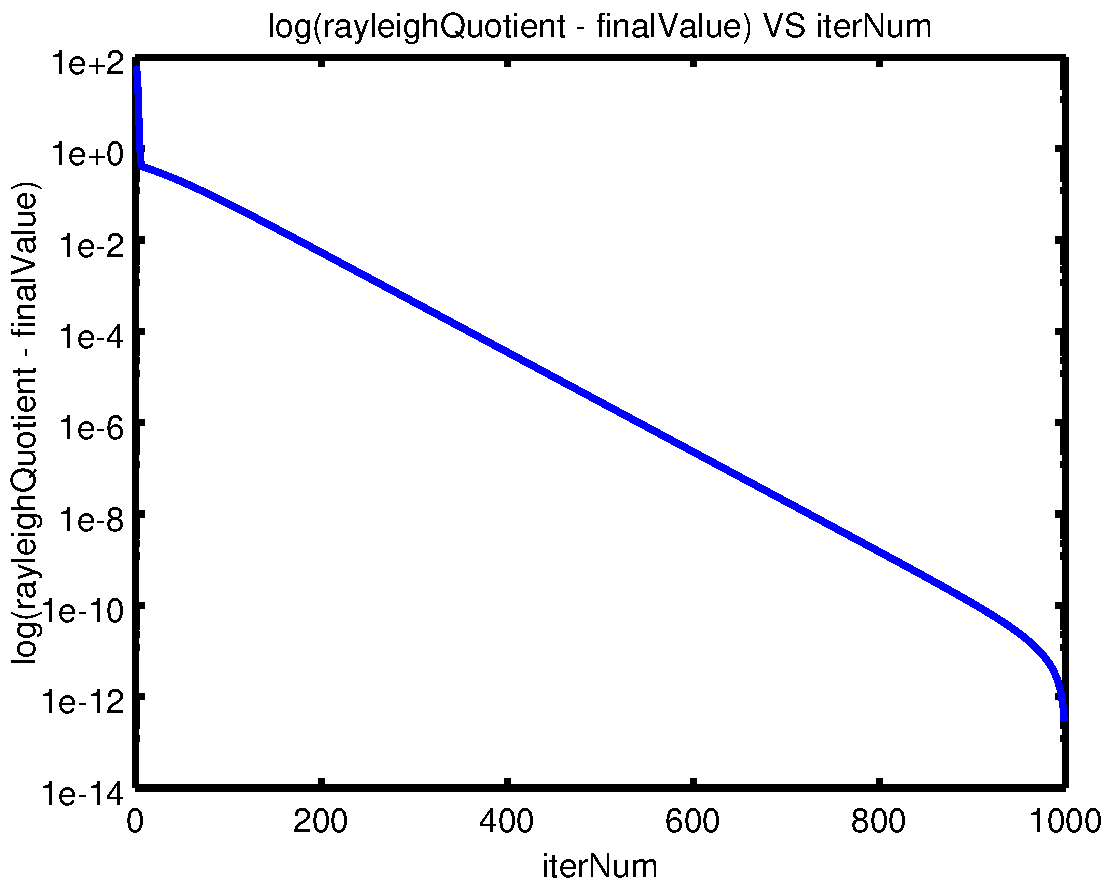
\includegraphics[scale=0.5]{./code/p1-crop.pdf}
  \caption{log(rayleighQuotient - finalValue) VS iterNum}
  \label{graph}
\end{figure}

\subproblem{b}
Rayleigh Quotient Iteration (RQI: inverse iteration with the shift at each step determined by the Rayleigh quotient with the iterate). Start with a random normalized vector. Which eigenvalue does it converge to? To force it to converge to the largest eigenvalue, apply RQI with a shift fixed at $A_{\infty}$ for a few initial iterations before switching to the pure Rayleigh quotient. How many initial iterations with fixed shifts do you need to make it converge to the largest eigenvalue? This number should be less than 10.

\solution
First we create a function \m{QRI} to implement the naive Qayleigh Quotient Iteration algorithm, and then we apply it to the test matrix.

\begin{lstlisting}
%% QRI Rayleigh Quotient Iteration to get the largest eigenvalue
%% Input matrix A; maximum iteration times t_max; eps0
%% Output eigenvector eigVec; eigenvalue eigVal; number of iteration iterNum; array of residuals for each iteration resArray

function [eigVec eigVal iterNum resArray] = QRI(A, iterMax, eps0)
  [n m] = size(A);
  eigVec = (rand(n, 1) - 0.5) * 2;
  [tmp1 tmp2] = max(abs(eigVec));
  eigVec = eigVec ./ eigVec(tmp2);
  eigVal = eigVec' * A * eigVec / (eigVec' * eigVec);
  B = (A - eigVal .* eye(size(A)))^(-1);
  iterNum = 1;
  resArray = zeros(iterMax, 1);
  resArray(iterNum) = norm(A * eigVec - eigVal * eigVec, 1);

  while (resArray(iterNum) > eps0 && iterNum < iterMax)
      eigVec = B * eigVec;
      [tmp1 tmp2] = max(abs(eigVec));
      eigVec = eigVec ./ eigVec(tmp2);
      eigVal = eigVec' * A * eigVec / (eigVec' * eigVec);
      B = (A - eigVal .* eye(size(A)))^(-1);
      iterNum = iterNum + 1;
      resArray(iterNum) = norm(A * eigVec - eigVal * eigVec, 1);
  end
end

n = 40
[Q,R] = qr(rand(n,n));
A = Q * diag([1:n-2,2*n-1,2*n]) * Q';
iterMax = 1000;
eps0 = 1e-07;
[eigVec eigVal iterNum resArray] = QRI(A, iterMax, eps0);

eigVal
% > 22.000
iterNum
% > 5
\end{lstlisting}

Here we see the algorithm converges within 5 steps. Note that the eigenvalue Rayleigh Quotient Iteration converges to is 22, not the largest one. In fact theoretically it's hard to say which eigenvalue the algorithm will converge to.

Next, we create a function \m{QRI\_f} to implement the modified Rayleigh Quotient Iteration algorithm, which fix the shift at $||A||_{\infty}$ for a few initial iterations before switching to the pure Rayleigh quotient.
\begin{lstlisting}
%% QRI_f Modified Rayleigh Quotient Iteration to get the largest eigenvalue
%% Input matrix A; maximum iteration times t_max; eps0, iterFix
%% Output eigenvector eigVec; eigenvalue eigVal; number of iteration iterNum; array of residuals for each iteration resArray

function [eigVec eigVal iterNum resArray] = QRI_f(A, iterMax, eps0, iterFix)
  fixShift = norm(A, inf);
  [n m] = size(A);
  eigVec = (rand(n, 1) - 0.5) * 2;
  [tmp1 tmp2] = max(abs(eigVec));
  eigVec = eigVec ./ eigVec(tmp2);
  eigVal = eigVec' * A * eigVec / (eigVec' * eigVec);
  B = (A - fixShift .* eye(size(A)))^(-1);
  iterNum = 1;
  resArray = zeros(iterMax, 1);
  resArray(iterNum) = norm(A * eigVec - eigVal * eigVec, 1);
  while (resArray(iterNum) > eps0 && iterNum < iterMax)
    eigVec = B * eigVec;
    [tmp1 tmp2] = max(abs(eigVec));
    eigVec = eigVec ./ eigVec(tmp2);
    eigVal = eigVec' * A * eigVec / (eigVec' * eigVec);
    if (iterNum < iterFix)
      B = (A - fixShift .* eye(size(A)))^(-1);
    else
      B = (A - eigVal .* eye(size(A)))^(-1);
    end
    iterNum = iterNum + 1;
    resArray(iterNum) = norm(A * eigVec - eigVal * eigVec, 1);
  end
end

n = 40;
iterFix = 10;
[Q,R] = qr(rand(n,n));
A = Q * diag([1:n-2,2*n-1,2*n]) * Q';
iterMax = 1000;
eps0 = 1e-07;
[eigVec eigVal iterNum resArray] = QRI_f(A, iterMax, eps0, iterFix);

eigVal
% > 79
iterNum
% > 14
\end{lstlisting}

Note that the algorithm converges within 14 steps.

Actually it's hard to say how many initial iterations with fixed shifts is needed to make it converge to the largest eigenvalue. We have tried different number of initial iterations and find that no matter which value you choose, you can't avoid the possibility that the algorithm may converge to some other eigenvalues. However, as the number of initial iterations grows up, the algorithm is more likely to converge to large eigenvalues, like 79 and 80 in this example.

\subproblem{c}
Simple explicit QR algorithm (no shifts). Try symmetrizing after each iteration. Allow up to 1000 iterations.

\solution
Here we create the function \m{QRAlgo} to implement the explicit QR algorithm.

\begin{lstlisting}
%% QR Algorithm to solve the eigenvalue eigenvector problem
function [eigVec eigVal iterNum resArray] = QRAlgo(A, iterMax, eps0)
  U = eye(size(A));
  iterNum = 1;
  resArray = zeros(iterMax, 1);
  A0 = A;
  [Q R] = qr(A);
  A = R * Q;
  U = U * Q;

  resArray(iterNum) = norm(diag(A0 * U - diag(diag(A)) * U), 1);
  while (resArray(iterNum) > eps0 && iterNum < iterMax)
    [Q R] = qr(A);
    A = R * Q;
    U = U * Q;    
    iterNum = iterNum + 1;
    resArray(iterNum) = norm(diag(A0 * U - diag(diag(A)) * U), 1);
  end
  
  eigVal = A;
  eigVec = U;
end

n = 40;
[Q,R] = qr(rand(n,n));
A = Q * diag([1:n-2,2*n-1,2*n]) * Q';
iterMax = 1000;
eps0 = 1e-07;
[eigVec eigVal iterNum resArray] = QRAlgo(A, iterMax, eps0);

iterNum
% > 1000 
\end{lstlisting}

Note that the QR algorithm does not converge within 1000 steps.

\problem{5}
Implement a simple Lanczos procedure (as given in the lecture notes, or Alg. 10.1.1 ∗ in the text or Alg. 36.1 in TB) to compute the factorization $AX = XT$ where $A$ is a given symmetric matrix, $X$ is a set of generated orthonormal columns, and $T$ is a generated tridiagonal matrix. Apply the procedure to the test matrices in the previous question and use the result to obtain a Ritz approximation (§10.1.4) to the leading eigenvalue/vector pair for $A$. You should use the standard simple Lanczos procedure, except that you should check for loss of orthogonality by the following heuristic: check that each generated Lanczos vector is orthogonal to the starting vector (i.e., the inner product is less than the given tolerance). Carry out the Lanczos expansion until n Lanczos vectors have been generated, or until an off-diagonal element of T is less than $10^{-7}$ (in absolute value), or until orthogonality is lost (to the same tolerance). Use a random starting vector.

Compute the Ritz approximation to the eigenvalue at each iteration, and plot the differences between the Ritz values and the final value as done with the Power Method above. You can also just compute the maximum eigenvalue of the leading $k \times k$ principal submatrix of the final T, for $k = 1, 2, \dots$ To obtain the Ritz values, just apply the built-in eig function to the tridiagonal matrix $T$ .

\solution
We first create a function called \m{lanczosTri} to implement the Lanczos procedure.
\begin{lstlisting}
%% lanczos Tridiagonalization, Given Matrix, AQ = QT, where Q is orthonormal and T is a tridiagonal Matrix
%% Input: n * n matrix A
%% output: orthonormal Q and tridiagonal T, s.t. AQ = QT

function [Q T] = lanczosTri (A, eps0)
    n = size(A, 1);
    beta = zeros(n + 1 ,1);
    alpha = zeros(n + 1, 1);
    Q = zeros(n, n + 1);
    R = Q;
    v = (rand(n, 1) - 0.5) * 2;
    v = v / norm(v, 2);

    k = 1;
    beta(1) = 1;
    R(:, 1) = v;

    while ((k == 1 || abs(beta(k)) > eps0) && k < n + 1)
        Q(:, k + 1) = R(:, k) / beta(k);
        k = k + 1;
        alpha(k) = Q(:, k)' * A * Q(:, k);
        R(:, k) = (A - alpha(k) * eye(size(A))) * Q(:, k) - beta(k - 1) * Q(:, k - 1);
        beta(k) = norm(R(:, k), 2);
        if abs((R(:, k) / beta(k))' * Q(:, 2)) > eps0
            break;
        end
    end

    Q = Q(:, 2 : (k));
    alpha = alpha(2 : (k));
    beta = beta(2 : (k - 1));
    
    T = zeros(k - 1);
    for i = 1 : k - 1
        T(i, i) = alpha(i);
        if (i < k - 1)
            T(i, i + 1) = beta(i);
            T(i + 1, i) = beta(i);
        end
    end
end
\end{lstlisting}

Then we try to apply function \m{lanczosTri} to the test matrix in the previous problem, compute the Ritz approximation to the eigenvalue at each iteration, and plot the differences between the Ritz values and the final value as done with the Power Method above.

\begin{lstlisting}
n = 40;
[Q,R] = qr(rand(n,n));
A = Q * diag([1:n-2,2*n-1,2*n]) * Q';
eps0 = 1e-07;
[eigVec eigVal iterNum resArray] = powerMethod(A, iterMax, eps0);
[Q T] = lanczosTri(A, eps0);
res = zeros(size(T, 1), 1);
for i = 1:size(T, 1)
  eigeig = max(eig(T(1:i, 1:i)));
  res(i) = abs(eigeig - eigVal);
end
semilogy(1:size(T,1), res)
hold on;
xlabel('iterNum');ylabel('Difference');title('Difference VS iterNum');
fontsize=20;
set([gca; findall(gca, 'Type','text')], 'FontSize', fontsize);
set([gca; findall(gca, 'Type','line')], 'linewidth', 3);
saveas(1, 'p2.pdf');
hold off;
\end{lstlisting}
\clearpage
We can see the differences between the Ritz values and the final value as done with the Power Method above in graph \ref{graph2}.

\begin{figure}[!ht]
  \centering
  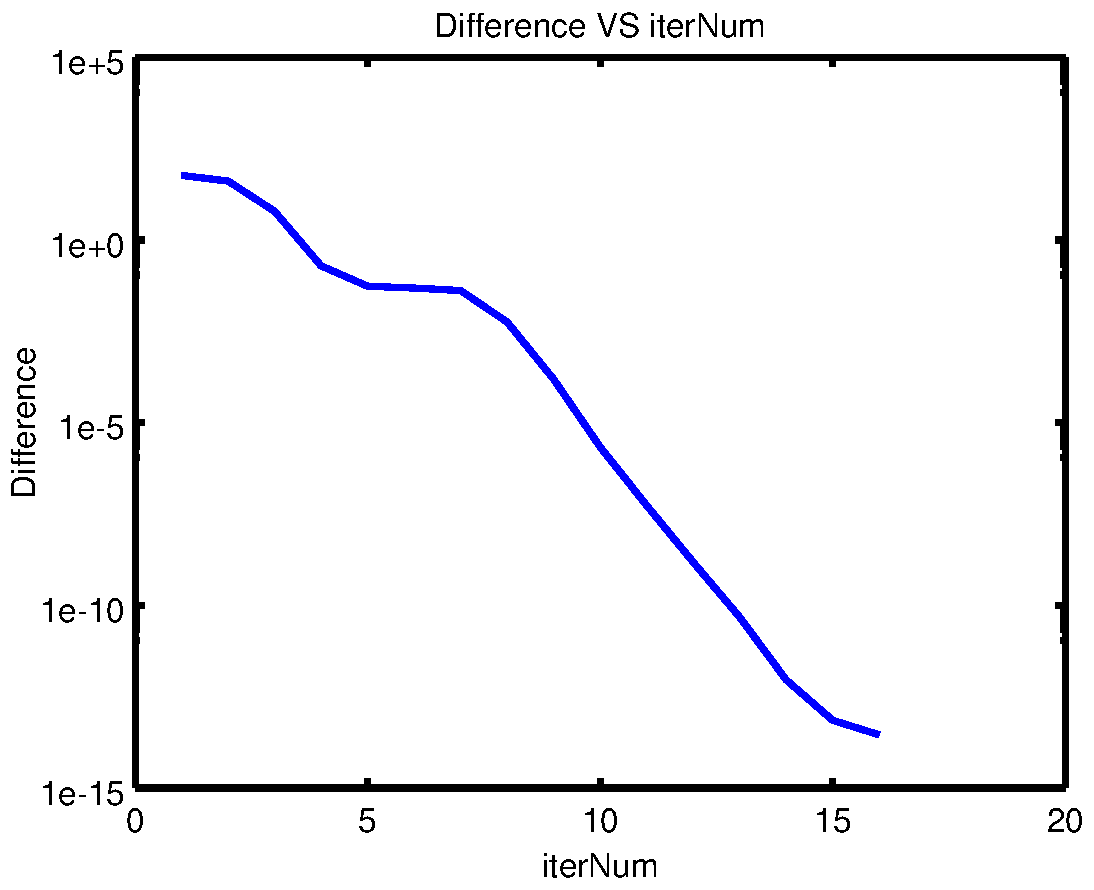
\includegraphics[scale=0.5]{./code/p2-crop.pdf}
  \caption{differences VS iterNum}
  \label{graph2}
\end{figure}


\end{document}